% Chapter Template

\chapter{State-of-the-art} % Main chapter title

\label{Chapter2} % Change X to a consecutive number; for referencing this chapter elsewhere, use \ref{ChapterX}

\lhead{Chapter 2. \emph{State-of-the-art}} % Change X to a consecutive number; this is for the header on each page - perhaps a shortened title

%----------------------------------------------------------------------------------------
%	SECTION 1
%----------------------------------------------------------------------------------------
\section{Introduction}

This chapter will discuss the research literature in the field of credit risk and default prediction of Small Medium Enterprises (SME/SMEs) customers in financial institutions. The first sections will cover off the areas of SME, detailing SME definitions, credit risk and how macro-economic features are utilised in modelling credit risk for SMEs and economies. These early sections will discuss challenges observed in the field such as a lack of shared definitions and statistics while it also details recommendations made to strengthen the field. The literature for macro-economic features is reviewed and it is noted that there is a dearth of research how macro-economic factors affect SME credit risk specifically and credit risk as a whole. The review concludes by detailing successful examples Italy and Portugal of applying macro-economic factors in predicting credit risk by utilising features based on default rates and unemployment by geographic location. 

The chapter will also review research literature in the field of knowledge discovery, data mining with a particular focus on predictive modelling. Knowledge discovery and data mining will be explained and illustrated with frameworks and methodologies around the approach to tasks in each. A review od the literature facilitates an understanding of the processes, prediction algorithms, feature selection methods, validation methods and performance measures required to build a predictive model to predict SME customers that are likely to default i.e. risky customers. A key observation emerging from  building a model to predict what customers will default is the tenancy towards a very large class imbalance in the dataset e.g. there will be a much larger proportion of good/well performing than bad/poorly performing customers. Methods of addressing this class imbalance are also discussed later in this chapter.

\section{SME Definition}
The most common definition for a SME is a registered business with fewer than 250 employees \citep{ifc_sme_2009}. However this definition is not universally agreed : there are variances in the definition between countries and even across financial institutions. 

At a European level a SME business is categorised as SME if they have two hundred and fifty people or fewer employed and if the annual turnover does not surpass \EUR50 million, and/or an annual balance sheet not surpassing \EUR43 million\footnote{\url{http://isme.ie/advice/sme-facts-faq}}\footnote{\url{https://www.enterprise-ireland.com/en/About-Us/Our-Clients/SME-Definition.html}}. SMEs can also be subdivided further into smaller subcategories. Micro enterprises are defined as businesses that employ fewer than ten people, have annual turnover below \EUR2 million, and annual balance sheet total not surpassing \EUR2 million. Small enterprises are defined as businesses employing between ten and fifty people, have annual turnover below \EUR10 million, and annual balance sheet total below \EUR10 million. Medium enterprises are defined as businesses with an employee number of between fifty and two hundred and fifty people, have an annual turnover less than \EUR50 million, and an annual balance sheet total below \EUR43 million\footnote{\url{http://www.cgap.org/financialindicators}}.

Worldwide, the most common method by regulators for defining businesses as SME are based on the number of people they have employed, sales/turnover or/and loan size \citep{ardic_small_2011}.

In 2004, at the Organisation for Economic Co-operation and Development (OECD) conference on SMEs, two key recommendations were made by member economies and non-member states\footnote{Second OECD Conference of Ministers Responsible for Small and Medium-Sized Enterprises (SMEs), Istanbul,2004. \url{http://www.oecd.org/cfe/smes/31919278.pdf}}: (i) develop SME statistics that can be compared internationally, and (ii) establish a common definition and set of rules for what is a SME. Without these statistics and definitions in place it would be more difficult to deploy programmes aiming to expand and strengthen the SME sector \citep{ardic_small_2011}. The aim of these recommendations is that, by having a consistent definition and statistics for SMEs, economies and analysts can learn from each other on a global scale with an end goal of building a stronger SME sector.


\section{Credit Scoring}

Financial institutions use classification systems called \textit{credit scoring} to evaluate the credit risks related with lending to a borrower. \textit{Credit risk} is the risk of losses expected when a borrower's ability or willingness to repay a financial obligation is adversely affected \citep{anderson_credit_2007}. \textit{Credit scoring} is the phrase used to encompass the methods and prediction techniques used by lenders to assess the credit risk of existing and prospective borrowers. 

The aim of credit scoring is to classify prospective borrowers and existing borrowers into one of two groups, good or bad. The bad group signifies a borrower who was deemed likely to default on the financial obligation. The good group signifies borrowers deemed likely to repay their financial obligation.

Credit scoring models are typically broken into two main categories, \textit{application scoring} and \textit{behavioural scoring}. The objective of the application scoring model is to predict at the time the application is made, the borrower's probability of defaulting at some time in the future. Application, product and demographic details are generally used to build the application scoring model. The objective of the behavioural scoring model is to predict the probability of existing customers defaulting. The borrower's repayment performance is mainly used to build the behavioural scoring model. 

Before credit scoring systems were employed by financial institutions, the risk of a borrower was based on the biased opinion of lender who would call on their life and work experience. Information about borrowers was gathered through personal relationships between borrowers and the employees of the lender \citep{anderson_credit_2007}. Further investigation was carried out by means of a process known as the 5Cs

\begin{enumerate}
	\renewcommand{\labelenumi}{(\roman{enumi})}  
	\item \textbf{Character} - does the borrower, or their family, have a relationship with the lender?
	\item \textbf{Capital} - what is credit amount requested?
	\item \textbf{Collateral} - is security being offered?
	\item \textbf{Capacity} - how fit is the borrower to repay?
	\item \textbf{Condition} - how is the economy performing presently?
\end{enumerate}

This process was clearly flawed as it would not offer the financial institutions any consistency or reliability in terms of to which borrowers it was lending. With large improvements in computer power in the 1980s financial institutions started utilising analytical methods to gain a deeper understanding of customer behaviour \citep{hand_modelling_2001}.

Credit scoring systems are imperfect solutions as they can only be used as estimates based on historic events or the pasts events, but not future events. A significant amount of debt goes unpaid each year due to the failure of credit scoring systems to identify borrowers who will default on their financial obligation \citep{finlay_multiple_2011}

Generally a credit scoring system is built using a credit scorecard. Scorecard points are added based on important borrower characteristics and a score is generated that represents the risk of that borrower relative to all the other borrowers, in order of who is most likely to default on their financial obligation.

The most basic credit scorecards consist of a set of features that are statistically supported to be predicting the credit risk of a borrower \citep{siddiqi_credit_2012}. One of the reasons for building a credit scorecard is for financial institutions to have a standardised, structured and easy to interpret mechanism of assessing borrower's credit worthiness.
 
The credit scorecard in Fig. \ref{fig:appScorecard} uses features such as age, previous banking history, credit card limits, years at current job, accommodation status, self-employed status and monthly income to assign \textit{Applicant X} a credit score. It can be seen in Fig. \ref{fig:appScorecard} that each feature is split into attributes and for each attribute a score has been generated which is added to the overall credit score for that applicant. 

\begin{figure}[H]
	\includegraphics[width=0.8\textwidth, center]{appScorecard}
	\caption{Application Scorecard for Applicant X with a Credit Score of 355	
	}
	\label{fig:appScorecard}
\end{figure}

It can be observed from Fig. \ref{fig:appScorecard} that high value attributes are associated with borrowers that are statistically thought to be less likely to default on a financial obligation. For example \textit{Applicant X} in the example had an overall score of 355; if there were another applicant, \textit{Applicant Y}, who had an overall score of 450, \textit{Applicant Y} would score higher and therefore less likely to default on the financial obligation than {Applicant X}.

%----------------------------------------------------------------------------------------
%	SECTION 2
%----------------------------------------------------------------------------------------
\section{Importance of Credit Risk Modelling for SMEs}
Recent research indicates that SME development is closely linked with economic growth. \cite{beck_smes_2005} indicates there are strong correlations between economic growth and the size of the SME sector in an economy. After the recent global financial crisis of 2008 and 2009 it is important to note that the SME segment is recognised as one of the most important factors contributing to sustainable employment and economic recovery \citep{lawless_smes_2012}. \cite{lawless_smes_2012} also note that this is mainly due to the indigenous, employment-intensive nature of SMEs. SMEs are of major importance to many economies; in Ireland SMEs account for 68 percent of employment and 99 percent of firms in the private sector \citep{lawless_irish_2012}. Since the financial crisis, SMEs have been hampered by restrictive policies and regulations, in their efforts to secure credit. However, it has been recognised internationally that credit constrained businesses engage with less economically valuable and growth-enhancing activity such as job and employment creation than similar unconstrained businesses \citep{campello_real_2010}. This means that financial institutions sit at the heart of the economy in making decisions about what businesses to give credit to. They will do this first to maximise their own profits but also promote growth leading to a sustainable employment sector and economy. This requires financial institutions' credit risk models take into account at all times the current economic factors that are influencing good and bad credit decisions. 

%----------------------------------------------------------------------------------------
%	SECTION 3
%----------------------------------------------------------------------------------------
\section{Macro Area Features Affecting SME and Economic Credit Risk}
\cite{hackbarth_capital_2006} note that even though there is a substantial amount of literature focussed on understanding and developing credit risk, there is a dearth of research into how macro-economic factors affect credit risk.  \cite{hackbarth_capital_2006} find it strange based on anecdotal suggestions from institutions that the economic business cycle is an important feature when calculating the probability of a customer defaulting. One example of this is that during a recession, consumers are less likely to spend money on discretionary goods or luxuries and as a result the credit risk of businesses in this sector will most likely rise due reduced demand from consumers. In \cite{hackbarth_capital_2006} they found that macro-economic conditions clearly have an impact on credit risk.

\cite{fama_term_1986} notes that over the counter derivatives broker-dealers measure risk using individual counter-parties' details but also make use of geographic data and performance indicators of other industry groups. The \cite{derivatives_policy_group_framework_1995} \footnote{The Derivatives Policy Group was made up of representatives of CS First Boston, Goldman Sachs, Morgan Stanley, Merrill Lynch, Salomon Brothers, and Lehman Brothers} also made recommendations that credit exposure was measured by geography and industry exposure when calculating credit risk.

Financial institutions can also suffer from a risk known as the \textit{winners curse}. In banking, this is a scenario where other financial institutions' credit risk models score a borrower too risky and will not lend to that applicant. That same borrower then arrives at ``our bank" where ``our model" scores them as a good or likely to repay borrower and decide to lend to them. As a result ``our bank" will take on an excessive amount of risk that where other banks' expected losses \citep{duffie_credit_2012}. \cite{duffie_credit_2012} also discuss how banks can mitigate their risk to the winners curse by including metrics such as borrowing rates and credit risk concentration limits by area or location.

Based on the Italian market, \citep{di_pietro_regional} investigated if SMEs experienced different levels of default rates based on the region in which they were located. They investigated the business cycles of these areas and looked at identifying which macro-economic features were the most influential in predicting default. For their experiment, they divided Italy into five areas, centre, north-east, north-west, south, and the islands. In their analysis, they confirmed that there was statistically a significant difference between default rates in different areas. This can be illustrated in Fig. \ref{fig:evolutionOfItalianDefaultRate}

\begin{figure}[H]
	\includegraphics[width=0.8\textwidth, center]{evolutionOfItalianDefaultRate}
	\caption{Evolution of the Italian SME Default Rate by Area (1985-2005) \\
	\cite[Source:][]{di_pietro_regional}		
			}
	\label{fig:evolutionOfItalianDefaultRate}
\end{figure}

From Fig. \ref{fig:evolutionOfItalianDefaultRate} one can see that the average default rate in the south of the country (green trend line) and islands (blue trend line) is significantly higher than in the north-west(red trend line) and north-east(orange trend line). They use the Kruskal-Walls test to confirm that the differences between the default rates are statistically significant.

In \cite{antunes_estimating_2005}, using Portuguese data, they found that macro-economic features such as the employment rate, short term interest rate and gross domestic product were useful when included in the predictive models to estimate the probability of default. Using these features allowed them to develop stress tests where they could run macro-economic scenarios that would have a negative affect on the economy. This is the same method that is widely adopted by the International Monetary Fund (IMF) in their Financial Stability Assessment Program (FSAP) which is used to assess a country's financial sector resilience and capacity to manage financial crisis. They produce tailored recommendations of a micro and macro nature based on each country's circumstances \citep{marston_financial_2001} 

\cite{ardic_small_2011} discusses how competition in developed countries and instability in developing countries provide some of the biggest challenges to modelling credit risk for SMEs. This view of developing counties is supported by research carried out by \cite{rocha_status_2011} which provides evidence from financial institutions in North Africa and the Middle East, detailing the immaturity of their financial systems and lack of SME transparency as some of the main obstacles. 


\section{Data Mining and Predictive Modelling}\label{sec:dataMining}
Knowledge discovery is defined by \cite{frawley_knowledge_1992} as the \textit{``as the non-trivial process of identifying valid, novel, potentially useful, and ultimately understandable patterns in data''}. Knowledge discovery can be thought of as extracting some piece of insight or value from data that could not have been done using a simple query. \cite{fayyad_knowledge_1996} outlined an approach called the Knowledge Discovery in Databases (KDD) which centres on extracting these useful patterns from data stored in large databases.

\begin{figure}[H]
	\includegraphics[width=0.8\textwidth, center]{kdd}
	\caption{Overview of the KDD process  \\
		\cite[Source:][]{fayyad_knowledge_1996}		
	}
	\label{fig:kdd}
\end{figure}

The goal at the end of the KDD process is to realise some value or extract some piece of insight. This is typically done through the data mining step of the process, but Fig. \ref{fig:kdd} above illustrates it is only one step in the overall framework of KDD. Steps such as data selection, pre-processing, transformation or data modelling must be completed prior to the data mining step. 


\begin{figure}[H]
	\includegraphics[width=0.4\textwidth, center]{crisp_dm}
	\caption{CRISP-DM Data Mining Process Model \\
		\cite[Source:][]{shearer_crisp-dm_2000}		
	}
	\label{fig:crisp_dm}
\end{figure}

There are methodologies and frameworks for data mining. One of these is the \textit{Cross Industry Standard Process for Data Mining}, usually referred to by CRISP-DM \citep{shearer_crisp-dm_2000}. This data mining framework is the one most commonly adopted by data miners to work out a problem. Some polls show it is the leading methodology used by data miners\footnote{\url{http://www.kdnuggets.com/polls/2014/analytics-data-mining-data-science-methodology.html}}. It can be seen in Fig. \ref{fig:crisp_dm}, that the CRISP-DM process is split into six main steps or tasks; \textit{business understanding}, \textit{data understanding}, \textit{data preparation}, \textit{modelling}, \textit{evaluation} and \textit{deployment}. The next most popular framework is known as Sample, Explore, Modify, Model and Assess more commonly known as SEMMA \citep{azevedo_kdd_2008}. This solution has been developed by Statistical Analysis System (SAS) institute but is seen more as a list of sequential steps that can be used to build out data mining solutions. The big advantage with the CRISP-DM methodology over SEMMA (illustrated in Fig. \ref{fig:crisp_dm}), is that it does not restrict one from moving between the different steps, and the arrow wrapping around the process suggests that even after deployment the process can continue.  


Since they were established over 20 years ago, the frameworks of KDD and CRISP-DM outlining steps to extract insights have grown and developed. There are a growing number of communities that continuously overlap. This can be illustrated below in Fig. \ref{fig:data_mining_venn_diagram}\footnote{\url{http://blogs.sas.com/content/subconsciousmusings/2014/08/22/looking-backwards-looking-forwards-sas-data-mining-and-machine-learning/}} where one can see that data mining, statistics, artificial intelligence and machine learning communities all share some common values. As a result, one can consider data mining as a
combination of KDD, machine learning, statistics and pattern recognition that may or may not leverage on databases. This results in the field of data mining being largely made up of data scientists, data analysts, computer scientists and statisticians \citep{coenen_data_2011}. 

\begin{figure}[H]
	\includegraphics[width=0.6\textwidth, center]{data_mining_venn_diagram}
	\caption{Data Mining Venn Diagram}
	\label{fig:data_mining_venn_diagram}
\end{figure}

For this research, the primary focus is on a subset of the data mining process called predictive modelling. This is represented in Fig. \ref{fig:crisp_dm}. Predictive modelling centres on predicting future events based on based on past or historic data. The predictions are trained using past real world events and are tested and evaluated on unseen real world data to see how they perform. 

Predictive modelling has many applications across a wide range of domains: some examples include election outcomes (\citep{silver_signal_2012}; \cite{tumasjan_predicting_2010}), predicting how oil slicks spread \citep{liu_tracking_2011}, cancer prediction \citep{delen_predicting_2005}, and recently predictive modelling has become popular in sports predictions of baseball \citep{lewis_moneyball_2004}, basketball \citep{stekler_predicting_2012} and horse racing \citep{silverman_predicting_2013}.
 

Financial institution commonly utilise predictive modelling across a variety of domains e.g. marketing and risk. In risk areas, banks will build predictive models to predict default probabilities for existing customers and evaluate customers applying for lending. This can reduce their risk, allowing them to increase profits meaning they can offer customers a better service and more personalised products. Thus credit scoring i s one of the most used application fields for data mining \citep{baesens_50_2009}.

Predictive models are built by using interval/numerical or/and categorical/nominal features/variables/predictors/attributes that can explain the target/class/outcome to be predicted. Once the model is trained on historic data, model performance and evaluation is carried out on unseen data for testing. The data used in training will not be the same as in test thus the model may not generalise well on unseen data. In the literature, this is known as model over-fitting on the training dataset. Methodologies, frameworks and testing can be put in place to mitigate the risk to this issue. These will discussed further throughout this chapter.

%----------------------------------------------------------------------------------------
%	SECTION 4
%----------------------------------------------------------------------------------------

\section{Dataset Construction}\label{sec:datasetConstruction}

Experts often detail how steps performed i n the data construction and preparation stage can be some of the most time consuming when building predictive models\footnote{For example see \url{http://www.kdnuggets.com/polls/2003/data_preparation.htm}}. There are many steps that need to be considered during the data preparation stage for building a prediction model that models credit risk of SMEs. Two that will be discussed in this section are the \textit{sampling period} and \textit{class label definition}. 

\subsection{Sampling Period}
As previously stated, predictive models are built using historical data. It must be acknowledged that past performance can be a useful predictor of defaulting but it does not guarantee that future predictions of the model will be accurate or reliable. A training dataset is built to train a predictive model where customers are observed at two different points in time \citep{martens_credit_2010}. They are observed at the time that the prediction is made based on past performance. They are then observed sometime in the future called the \textit{default observation point} at which they will classified by the model as good or bad. The amount of time between these two points is commonly known as the \textit{outcome window}. The length of the outcome window can vary based on business objectives and requirements. The industry standard in \subjectname\ dictates that this is usually 12 months. 

\subsection{Class Label Definition} \label{classLabelDef}
Defining a customer as defaulted is dependant on the objective of the particular predictive model and the requirements of the financial institution \citep{mcnab_principles_2000}. The Basel II definition (paragraph 452) which is widely used by financial institutions, including \subjectname\, considers a default to have taken place when either or both of the following criteria are met:
\vspace{-3mm} 
\begin{itemize}
	\item The bank/financial institution considers that the obligor is unlikely to pay its credit obligations to the banking group in full, without recourse by the bank to actions such as realising security (if held).
	\item The obligor is past due more than 90 days on any material credit obligation to the banking group. Overdrafts will be considered as being past due once the customer has breached an advised limit or been advised of a limit smaller than current outstandings.
\end{itemize} 

According to \cite{anderson_credit_2007}, there are two well known approaches to class label definition that financial institutions can choose: (\textit{i}) a \textit{current status} label definition which classifies a customer to have defaulted or not at the end of the outcome window or (\textit{ii}) a \textit{worst status} label definition which classifies whether the customer has defaulted or not throughout the outcome window. It is \subjectname's industry standard to use the \textit{worst status} option. This is in keeping with Basel II \citep{basel_international_2006}, that customers' 90 days worst status covering a one-year period is considered the standard definition for customers who have defaulted. 


\subsection{Segmentation}\label{sec:segment}
Segmentation is carried out by splitting the dataset population into multiple groups and building a prediction model for each group \citep{myatt_making_2007}. This splitting will be carried out using group specific criteria and allows for modelling characteristics and features that are important to each group independently.

For marketing, \cite{wedel_market_2012} illustrate how segmentation can be utilised to collate customers into homogeneous groups based on those customers' buying pattens and demographic data like location, age and income.

Segmentation can be used in credit scoring to allow the lender to have more flexibility when personalising credit products for customers, for example interest rate and repayment structure\citep{kennedy_credit_2013}.

Segmentation is carried out by analysts who generally require both subject matter expert experience and by leveraging statistical methods \citep{siddiqi_credit_2012}


%----------------------------------------------------------------------------------------
%	SECTION 5
%----------------------------------------------------------------------------------------
\section{Predictive Models}\label{sec:predictModels}
This section details some of the classification algorithms that can be used when modelling a binary classification problem. For this thesis the problem is if a customer defaulted or did not default on their financial obligation; hence, it is a binary classification problem. The algorithms discussed in this section are not an exhaustive list but all are suitable for use in the financial industry. Classification models discussed include linear and logistic regression, k-nearest neighbour (KNN), support vector machines (SVM) and neural networks. 

Based on research and experience working in industry, logistic regression is one of the most widely used classification algorithms used by industry.

\subsection{Regression} \label{Reg}
Regression models are used to model the linear relationship between features in a feature space or between the features and the target variable.

A very simple form of linear regression is where there is one independent and one dependent variable, which is the target one is attempting to predict. The model is often represented by the following equation

\begin{equation} \label{eq:reg}
	\text{Linear Model} = y = b_0 + b_1x
\end{equation}

where the model is trying to predict $y$ using the value of $x$.

Fig. \ref{fig:simpleLinearRegression} illustrates a very simple real life example of linear regression. It demonstrates the linear relationship between a person's heights and a person's weight.

\begin{figure}[H]
	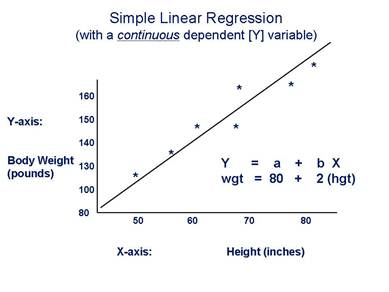
\includegraphics[center]{simpleLinearRegression}
	\caption[Confusion Matrix]
	{Simple Linear Regression}
	\label{fig:simpleLinearRegression}
\end{figure}

It can be seen from the above that $y$ in this example is weight (wgt) and $b_0 + b_1x$ is $80 + 2*Height(hgt)$ is what we are using to predict $y$. This is a very basic example but demonstrates how this can be leveraged for more complex feature sets. Predicting arrears is a dichotomous problem meaning the outcome of the experiment can only have two possible values. 

\subsection{Logistic Regression} \label{LogReg}
\textit{Logistic Regression} \cite[See:][]{hosmer_applied_2000} within the credit scoring industry is one of the most used algorithms \citep{hand_evaluating_2010}. As seen above in Fig. \ref{fig:simpleLinearRegression}, a simple regression model outputs a continuous response, in the given example it is body weight. Credit scoring or predicting arrears is a problem where there can only be two possibly values default or not-default. To simplify, this is reduced to a binary problem where the outcome will be 1 or 0 \citep{zou_modified_2004}. To transform the output of a regression model from $[-\infty, +\infty]$ to a probability between 0 and 1, a logistic transformation is applied. The logistic function can be used to take any value between $+\infty$ and $-\infty$ and output a value between $0$ and $1$. Fig. \ref{fig:logistic_function} below illustrates what a logistic function looks like.


\begin{figure}[H]
	\includegraphics[width=0.6\textwidth, center]{logistic_function}
	\caption[Standard Logistic Regression]
	{Standard Logistic Regression}
	\label{fig:logistic_function}
\end{figure}

The logistic function is defined in Equation \ref{eq:logitReg} as the following: 

\begin{equation} \label{eq:logitReg}
	\text{Logistic Model}  =  p  =  \frac{1}{1 + e^{-(b_0 + b_1x)}}
\end{equation}

As discussed previously, linear regression is an unsuitable classifier for making dichotomous predictions as linear regression produces predictions for a range beyond 0 to 1. Logistic regression also produces a curved line that is bounded by values between 0 and 1 (See Fig. \ref{fig:LogRegVsLineReg}).

\begin{figure}[H]
	\includegraphics[width=0.6\textwidth, center]{LogRegVsLineReg}
	\caption{Comparison between Linear and Logistic Regression Models}
	\label{fig:LogRegVsLineReg}
\end{figure}

In Fig. \ref{fig:LogRegVsLineReg} the constant, $b_0$ dictates the position of the curve which can be moved left and right depending on its value, $b_1$ will be the slope of the curve. 

The logistic regression model can be extended to include any number of interval and nominal features. This is illustrated in Equation \ref{eq:logitRegExtended}.

\begin{equation} \label{eq:logitRegExtended}
	p  =  \frac{1}{1 + e^{-(b_0 + b_1x_1 + b_2x_2 +\cdot\cdot\cdot+ b_px_p )}}
\end{equation}

Logistic Regression can also be used in cases where there are more than two outcome groups. For example, it could be used in predicting at what stage a customer is in the customer lifecycle e.g. Awareness, Interest/Consideration, Evaluation/Purchase. This is referred to as \textit{multinomial logistic regression}.


One of the main major attractions of logistic regressions is that it allows one to use discrete, continuous features or a combination of both \citep{lee_application_2005}.

\subsection{K-Nearest Neighbour} \label{kNN}
The \textit{k-nearest neighbour}, or {k-NN} for short, is an algorithm that classifies observations based on how its nearest neighbours are classified. It can be known as the nearest neighbour but in the majority of cases it is useful to use more than one neighbour \citep{henley_k-nearest-neighbour_1996}. The intuition behind this algorithm is that instances which are close by each other will more likely be classified the same way \citep{cover_nearest_1967}. We can see in Fig. \ref{fig:KNN_Example}\\ %added space for small gap in picture 


\begin{figure}[H]
	\includegraphics[width=0.6\textwidth, center]{KNN_Example}
	\caption{Example k-NN, Contrasting Results for \textit{k}=3 and \textit{k}=5 }
	\label{fig:KNN_Example}
\end{figure}

that results of the algorithm can vary with the choice of \textit{k}. It should also be noted that when applying this algorithm to a binary experiment, it is good practice to choose only odd values of \textit{k}, as this will eliminate the risk of ties from the decision process \citep{keller_fuzzy_1985} 

While adopting the k-NN algorithm there are multiple methods to decide what are your nearest neighbours. There are some common distance measures for continuous features only. Equation \ref{eq:Minkowski} is the \textit{Minkowski distance}, which is one of the most common, where \textit{p=1} this becomes the Equation \ref{eq:Manhatten}, the \textit{Manhatten distance}, and where \textit{p=2} this becomes the Equation \ref{eq:Euclidean} the \textit{Euclidean distance}.

\begin{equation} \label{eq:Minkowski}
	\text{Minkowski Distance}   = \Big(\sum_{i=1}^k (\abs{x_i-y_i})^p\Big)^\frac{1}{p}
\end{equation}

\begin{equation} \label{eq:Manhatten}
	\text{Manhatten Distance}   = \sum_{i=1}^k \abs{x_i-y_i}
\end{equation}

\begin{equation} \label{eq:Euclidean}
	\text{Euclidean Distance}   = \sqrt{\sum_{i=1}^k (x_i-y_i)^2}
\end{equation}

The results from k-NN will vary depending on your choice of distance measurement. There are also other distance metrics for continuous features such as \textit{Correlation Similarity} and \textit{Cosine Similarity} \citep{sarwar_item-based_2001}

Through analysis one can evaluate the optimal value for \textit{k}, one based on inspecting the results and creating benchmarks. Anecdotally, the larger the value of \textit{k} the more precise the algorithm can be but as with most things in data mining there are no guarantees. Choosing a high $k$ could also potentially cause over-fitting of the training data.

\subsection{Decision Trees} \label{decTrees}
The \textit{decision tree} algorithm classifies observations into classes in the form of tree-like structure, hence the name. The algorithm seeks to partition the dataset into smaller subsets, using the relationship between the feature set and target variable to do so. An example of a simple decision can be seen in Fig. \ref{fig:decisionTree}

\begin{figure}[H]
	\includegraphics[width=1\textwidth, center]{decisionTree}
	\caption{Simple Decision Tree for Yes, No Prediction \\ \cite[Source:][]{quinlan_induction_1986}}
	\label{fig:decisionTree}
\end{figure}

The output of the algorithm splits the data into smaller subsets of data; the output is a tree with a root node, internal nodes and leaf nodes. As can be seen in Fig. \ref{fig:decisionTreeExplained}, the root node in this example \textit{`Outlook'} is the first node in the tree which means it is the most predictive feature. 

\begin{figure}[H]
	\includegraphics[width=.6\textwidth, center]{decisionTreeExplained}
	\caption{Decision Tree with Nodes and Leaves labelled}
	\label{fig:decisionTreeExplained}
\end{figure}

The \textit{root node} will have have two or more branches. In this case, there are three \textit{`Rainy', `Overcast'} and \textit{`Sunny'}. Below these branches there are \textit{internal or split nodes} \textit{'Windy'} and \textit{`Humidity'} which in turn output more branches. The bottom nodes of each decision or branch is the prediction or classification, this is called the \textit{leaf node}. In this example the leaf node decision will be whether or not it will rain represented by Yes/No in Fig. \ref{fig:decisionTreeExplained}.

The algorithm that builds decision trees is called the \textit{iterative dichotomiser 3} or more commonly known as ID3 \citep{quinlan_induction_1986}. The algorithm applies a top down approach to choosing its root and internal nodes. The algorithm only evaluates one step ahead from where it is in the decision process at any time and does not allow for any backtracking. This decision making process is known as a greedy approach as it just makes the optimal solution at that particular stage of the process. Due to these limitations, the optimal solution is not guaranteed \citep{friedman_lazy_1996}.

The ID3 algorithm works by calculating the \textit{entropy} and \textit{information gain} at each step or decision node, where one uses the feature with the smallest entropy or feature that maximises information gain.

Entropy $H(S)$ seen in Equation \ref{eq:entropy} measures how much uncertainty there is in the data \citep{shannon_mathematical_2001}

\begin{equation} \label{eq:entropy}
	H(S) = - \sum_{x \in X} p(x) \log_{2} p(x)
\end{equation}
Where:
\begin{itemize}[label=]
	\item $S$: The current dataset for which entropy is being calculated, this will change each time entropy is calculated
	\item $X$: The set of classes in $S$
	\item $p(x)$: Proportion of observations in class $x$ compared to total number in set $S$
\end{itemize}
If $H(S) = 0$ then the observations in $S$ are all of the same class. Entropy is calculated for each feature and the feature with the smallest entropy is used to split at that step.

Information gain is used to measure the decrease in entropy after the dataset is split on a feature. The equation for the information is 

\begin{equation} \label{eq:infoGain}
	IG = H(S) -  H(T)
\end{equation}
Where:
\begin{itemize}[label=]
	\item $H(S)$ is the the entropy of S
	\item $H(T)$ is the entropy of subset T based on splitting data on some feature
\end{itemize}

Information gain is calculated and the feature with the highest information gain is chosen to split the dataset. The algorithm then runs recursively until all the data is classified and predictions have been made. 

Multiple decision trees may output the same results. This can be seen in Fig. \ref{fig:simpleComplex} where two different decision trees classify the dataset correctly. \cite{quinlan_induction_1986} suggests that that in scenarios like this, the simpler decision tree would be chosen (Fig. \ref{fig:simple}).

\begin{figure}[H]
	\centering
	\begin{subfigure}[b]{0.45\textwidth}
		\captionsetup{font=scriptsize}
		\includegraphics[width=\textwidth, height=5cm]{decisionTreeSimple}
		\caption{Simple Decision Tree}\label{fig:decisionTreeSimple}
		\label{fig:simple}
	\end{subfigure} ~\quad
	\begin{subfigure}[b]{0.45\textwidth}
		\captionsetup{font=scriptsize}
		\includegraphics[width=\textwidth,height=5cm]{decisionTreeComplex}
		\caption{Complex Decision Tree}\label{fig:decisionTreeComplex}
		\label{fig:complex}
	\end{subfigure}
	\caption{Simple and Complex Decision Tree Comparison\\\cite[Source:][]{quinlan_induction_1986}}
	\label{fig:simpleComplex}
\end{figure}

This is done because the simpler the rules of the tree the more likely the tree is to generalise well on unseen data. In other words, if the tree is too complex it is more than likely over-fitting the training dataset. There is also a computational cost to classifying complex algorithms. 

 Other issues one needs to be mindful of when building a classifier using a decision tree include the following. Information gain can be biased to features that have a large number of values. These features will result in a root node that produces a very broad or wide tree which classifies the training data well or perfectly but performs very poorly on unseen cases. One scenario where this could happen would be if one used the unique identifier of each record  as a training input; this model would perform very well in training but would not perform well on unseen data. There are methods to mitigate the risk of over-fitting against these features such as \textit{gain ratio}, \textit{symmetric uncertainty} and the \textit{Gini index}. \cite{quinlan_induction_1986} noted that using these methods for node decision often produced favourable results when compared with information gain. It should also be noted that \textit{gain ratio}, \textit{symmetric uncertainty}, \textit{Gini index}, and \textit{information gain} can be used in the feature selection process which is discussed in Section \ref{sec2:featureSection}.

\subsection{Artificial Neural Networks} \label{neuralNets}
The \textit{artificial neural network} (ANN) is a learning algorithm based on an understanding of how neural networks, such as our brains, learn. Motivation to study how an ANN works comes from the success of how the human brain is faster than the worlds' fastest computers at certain applications such as object recognition, speech recognition and general perception \citep{haykin_neural_1998}.

As a human grows, their brain develops, learns and creates a set of rules based on the experiences it has had. These rules and experiences are stored in approximately 100 billion neurons or nerve cells in the brain. These neurons are connected in a network and use this as a method of communication, sending electrical and chemical signals back and forth between each other. On their own, each neuron is not very useful but in combination with other neurons and communication, this has allowed humans to learn and grow so successfully. 

An ANN seeks to replicate the neural network of the human brain, albeit on a much smaller scale. It does this by taking advantage of powerful computers which carry out a lot of simple tasks very quickly. ANNs have proven their value from their ability to map out any non-linear function \citep{white_learning_1989} and their prowess in applications such as pattern and speech recognition and forecasting \citep{kaastra_forecasting_1995}.

Fig. \ref{fig:annFotwardFeeding} shows a common layout of an ANN. As in the human brain, the ANN is comprised of processing neurons usually known as nodes which are organised into three layers, input, hidden and output. Nodes are connected between layers and as seen in Fig. \ref{fig:annFotwardFeeding} each connection may carry a different weight.

\begin{figure}[H]
	\includegraphics[width=.6\textwidth, center]{annFotwardFeeding}
	\caption{Three-layered Feed-forward Artificial Neural Network Configuration \\
				\cite[Source:][]{raju_development_2011}
			}
	\label{fig:annFotwardFeeding}
\end{figure}

Data comes in through the input layer's nodes and is fed through the network, from the input to the hidden and then onto the output layer. In the hidden layer, each node calculates a sum based on the input node and the weight of the connection. These hidden nodes then pass on values to the nodes in the outer layer where another calculation is performed: this calculation converts the value to a value between 0 and 1 by passing it through the sigmoid function seen in Fig. \ref{fig:logistic_function}. Throughout the training process, the connection weights are changed and tested in order for the ANN to learn and improve its predictions \citep{haykin_neural_1998}

ANNs have become increasingly popular in recent years due to improvements in the algorithms, the increase in computer power and success in application such as object and speech recognition. However, some remain sceptical because of the ``black box" nature of their results, where users do not know what the internal workings of the algorithm are  \citep{kaastra_forecasting_1995}. 



\subsection{Support Vector Machines} \label{SVM}
A Support Vector Machine (SVM) algorithm was developed first by \cite{vapnik_nature_1995}. The algorithm performs classifications via a hyperplane in a higher dimensional feature space that maximises the margin or distance separating the two classes. It can be seen in Fig. \ref{fig:svmExample} that the two classes are linearly separable using the hyperplane in the higher dimensional feature space. 

\begin{figure}[H]
	\includegraphics[width=.5\textwidth, center]{svmExample}
	\caption{Optimal Separating Hyperplane in SVMs of Feature Space \\
		\cite[Source:][]{li_adaptive_2011}
	}
	\label{fig:svmExample}
\end{figure}

SVM handles situations of non-linear data by using kernel functions (non-linear) to transform the data into a higher dimensional feature space. This allows it to become linearly separable via a hyperplane, this is known as the \textit{kernel trick}. This is illustrated in Fig. \ref{fig:svm_nonLinearlySeperable}, where non linearly separable data is transformed into a higher dimensional feature space where it can be linearly separated using a hyperplane. This ability is what differentiates SVM from logistic regression.

\begin{figure}[H]
	\includegraphics[width=.5\textwidth, center]{svm_nonLinearlySeperable}
	\caption{SVM Classifying Non-Linearly Classes \\
		\cite[Source:][]{burges_tutorial_1998}
	}
	\label{fig:svm_nonLinearlySeperable}
\end{figure}

There is much documentation illustrating the successful application of SVMs in several domains, including areas such as credit risk evaluation \citep{van_gestel_credit_2009} and text categorisation, cancer diagnosis and pattern recognition \citep{shin_application_2005}.

\subsection{Ensemble Models and Boosting} \label{boosting}

In 1907, mathematician Sir Francis Galton went to a market in which there was a challenge
to approximate the weight of an ox. After evaluating the 787 forecasts made by the
participants, he noticed that while there was a large variance in the forecast from the correct weight, the median value of the
forecasts was less than 1\% away from the correct weight of the Ox \citep{galton_vox_1907}. Although separate forecasts failed miserably, the united wisdom of the every guess generated a very accurate estimate. This is similar to how ensemble models are generated.


Boosting relates to a powerful principal of generating a very accurate prediction model using an aggregation of reasonably inaccurate ``rules of thumb'' \citep{freund_short_1999}. A frequently utilised ensemble is the Adaptive Boosting algorithm which is frequently called AdaBoost in the literature. A weak learner is produced from the first iteration where all of the observations can potentially be chosen. For later sampling of the distribution, the model makes adjustments based on the error rates of the classifier, so that model only will look at samples of data that were incorrectly classified \citep{freund_short_1999}. In this way, the algorithm is adopting step by step, based on the errors of past classifications and then focuses on correcting the record labels it got incorrect. A specific method of AdaBoost is the Boosted-Stumps Model. This is an ensemble model that leverages decision tree stumps, which are decision trees with one split. This method is seen to be optimal compared to the common AdaBoost model which tends to over-fit the training dataset \citep{caruana_empirical_2006}.

Bagging is an alternative method employed to generate ensemble models leveraging decision trees. One method of bagging is \textit{bootstrap replica}. This method works on the principle for a dataset of size $n$ to be used to train a model, generating trees using just different partitions of the training data with replacement \citep{dietterich_experimental_2000}. 

Random forests are another example of an ensemble model generated using multiple decision trees. A large number of decisions trees will be trained and results are combined together to make a classification, hence why it is called a `forest'. Each decision tree is trained on random subsets of the features available, hence why its called a `random' forest. Research provided by \cite{breiman_random_2001} demonstrated that the random forests performed better on tests compared to the AdaBoost method across a variety of datasets.


\section{Feature Selection}\label{sec2:featureSection}
Feature selection is a process of choosing the best subset of features from the full dataset to train the prediction model. \cite{guyon_introduction_2003} discusses that feature selection methods are usually split into one of three categories (i) filter techniques (ii) wrapper techniques and (iii) embedded techniques. 

\subsubsection{Filter Methods}
Filter feature selection methods use statistics to assign a score for each feature versus the target. The features are then ordered by predictability and a decision is made as to what features to keep. Filter method techniques include information gain, correlation coefficient and the chi squared test.

\subsubsection{Wrapper Methods}
Wrapper feature selection methods evaluate various subsets of features together while scoring the model for each subset. The resultant different model results are then evaluated and compared against the other results, returning the result which offered the best score based on the model evaluation criteria. Forward, backward and general stepwise regression are very common techniques of wrapper methods.

\subsubsection{Embedded Methods}
Embedded feature selection methods attempt to combine the two previous methods. That is, the method looks to learn what features are useful as the model is being created. 

Feature selection is very important in the credit scoring process and there are many reasons in the literature that suggest it should be used. The \textit{curse of dimensionality} is one such issue. If there are too many features in the model, it may perform well on the training dataset but when executed on unseen data it may perform poorly because the model has over-fitted many irrelevant or noisy features \citep{loughrey_overfitting_2005}. Research from (\cite{thomas_consumer_2009}; \cite{mays_credit_2004}) advises that to build a robust scoring model there should be somewhere between 8 and 20 predictive features. There are many reason for this: there is a practical issue of having to model more features; there are costs, overheads and maintenance associated with each redundant feature in the model. Referencing Fig. \ref{fig:simpleComplex}, one can see that it is much more desirable to have a simple decision tree than a complex decision tree with the same outputs. Similarly, if two datasets are providing the same results and one is a subset, it is always better to choose the subset. 

\section{Coarse Classification} \label{sec:binning}
Coarse classification is often utilised to transform the predictive features into a simpler form which is better suited for modelling \citep{carroll_transformation_1988}. Coarse classification is also referred to in the literature as binning, grouping or discretisation. For continuous and categorical features, values are transformed into a small number of bins or groups. These values  are mapped into these groups by referring to the target feature to identify the optimal cut-off points. 

Coarse classification has many benefits, one of which is that it allows for capturing the features' non-liner relationship with the target feature. This is achieved by each category in the group being treated as its own dummy variable which will have its own weight in a logistic regression model \citep{hand_optimal_2005}. Coarse selection can also increase the overall robustness of the model by reducing the possibility of over-fitting. It does this by creating groups with the optimal number of good records \citep{baesens_50_2009}. It also offers the capability of mitigating against the risk of outliers and missing values. 

Coarse classification is also very quick to deploy. Previously, it would have been achieved by analysts iteratively completing the process which was a very time consuming. Algorithms now such as chimerge and recursive partitioning to name a few, find optimal cut-points in the features quickly and accurately. These groups are then evaluated using the \textit{Weight of Evidence} (WoE) and \textit{Information Value} (IV) \citep{garcia_survey_2013}. 

A common methodology in coarse classification is to break up each feature into roughly three to six bins or groups \citep{hand_optimal_2005}. It is recommended that bins are limited to six to ensure the model does not become over-parameterised and difficult to manage. Conversely, the model will become too rigid if fewer than three groups are used. 

Approximating the WoE of each bin and tuning where optimal is the most-known method in carrying out coarse selection \citep{thomas_consumer_2009}. In a credit scoring problem the WoE for bin $i$ is defined as 
  
\begin{equation} \label{eq:woe}
\text{WoE} =  \ln\bigg(\frac{n_g(i)}{n_b(i)} \bigg/ \frac{N_g}{N_b}\bigg)
\end{equation}

where the amount of goods in a bin $i$ is $n_g(i)$, and the amount of bads in a bin $i$ is $n_b(i)$. $N_g$ and $N_b$ are the total amount of goods and bads in the full dataset. A negative WoE signals that a bin is more likely to default, whereas a positive WoE signals they are likely to not default.

The information value is frequently applied with the WoE. The IV is a powerful method for ranking variables by their importance which can be used for feature selection in the prediction model. The IV suggests the predictive capability of a binned feature and is defined as  
 
\begin{equation} \label{eq:informatoValue}
\text{IV} =  \sum\limits_{i=1}^j \bigg(\frac{n_g(i)}{N_g} -   \frac{n_b(i)}{N_b}\bigg) * \text{WoE$_i$}
\end{equation}

where $j$ is the number of bins in a feature. The IV of each bin is known as a contribution, which are then added together to generate the IV of a feature.

In general, binned features with an IV between 0.3 and 0.5 are thought to be very predictive features \citep{mays_credit_2004}. If the IV is more than 0.5 it could be an anachronistic feature and should be examined further \citep{siddiqi_credit_2012}. Binned features with an IV smaller than 0.1 are thought to be weaker features and their removal from the model should be considered \citep{anderson_credit_2007}.

\begin{comment}
\subsection{Correlation-based Feature Selection}
\subsection{Information Gain}
\subsection{Coarse Classification/ Binning}
\end{comment}

\section{Class Imbalance Problem}\label{sec:imBalance}
A key assumption which needs to be taken into account when using classification algorithms is that there is a balanced distribution of the target class \citep{japkowicz_class_2000}. Target class imbalance is described by  \citep{chawla_smote:_2002} where the number of records in each class are not equal. In a balanced dataset, the ratio between the a binary target class would be close to 50:50. 

One of the issues with imbalance arises when algorithms assume there is a balanced target class and they attempt to maximise the accuracy by predicting the most common class \citep{drummond_severe_2005}. The algorithms attempt to minimise the classification errors but fails to account for the incorrectly classifying cases \citep{seiffert_improving_2009}. While the overall classification might be very accurate, the results are not very useful in real world problems. This is because, in most cases, the algorithm will focus on the majority class, because of how heavily it is weighted in the training dataset and therefore ignoring the minority class. This is a serious issue because in most situations, the aim will be to predict the minority class. In this thesis, SME customers going into default is the minority e.g. there are more SME customers who do not default at the end of the outcome window than SME customers who default.

In recent years, more of the data mining and machine learning literature has explored the issue of class imbalance. \cite{weiss_mining_2004} discusses the role and issues that rare class instances can play in data mining. \cite{weiss_mining_2004} makes the distinction that there are two types of class imbalance which depend on the type of rarity in the data, these are called \textit{absolute rarity} and \textit{relative rarity}.

The primary issue with rarity is that there is simply a lack of data in real world problems. Absolute rarity occurs when the number of instances related to the rare class is very small in an absolute sense. Lack of data means it is difficult to identify what leads to a rare class. Fig. \ref{fig:absoluteRarity} illustrates how absolute rarity can pose difficulty.

\begin{figure}[H]
	\includegraphics[width=0.6\textwidth,center]{absoluteRarity}
	\caption{
		Impact of Absolute Rarity in Data Mining \\ \cite[Source:][]{weiss_mining_2004}
	}
	\label{fig:absoluteRarity}
\end{figure}

On the left side of Fig. \ref{fig:absoluteRarity} there is only one rare/positive example, compared to the right where there is more data thus more rare cases. It can be observed that the decision boundary on the right side of Fig. \ref{fig:absoluteRarity} is much more accurate when there is more data than on the left side Fig. \ref{fig:absoluteRarity} when there is just one observed rare class. This is a simple illustration of the fact that more data should facilitate better predictions. Relative rarity is where classes are not rare in an absolute sense but are rare relative to other objects. A supermarket example can illustrate this better: imagine trying to identify the relationship between two items but these items are rarely purchased as a whole, so even if they happen to be purchased together, the relationship may be difficult to identify.

As previously mentioned, class imbalances in the dataset occur very often in real world problems and thus research has been devoted to proposing methods of mitigating against this risk. \cite{chawla_editorial:_2004} proposed solutions centres on fine tuning the algorithm and manipulating the data. 

\subsubsection{Manipulating the data} \label{sec:dataManip}

A method of manipulating the data is to resample the data with the aim of balancing the distribution of the target class. Solutions proposed are as follows:

\begin{itemize}
	\item Random undersampling of the majority class
	\item Random oversampling of the minority class
	\item Synthetic sampling of the minority class 
\end{itemize}

A method commonly used is to randomly oversample the minority class in the training set. However, this increases the chances of over-fitting the algorithm to the training data as the model has been trained on multiple copies of the same data, none of which are adding any new information. This may cause the trained model to be biased and skewed on the training data, causing it to perform poorly on the test data \cite[See][]{hawkins_problem_2004}.

Random undersampling of the minority class is where random samples of the training dataset that are part of the majority class are removed. This means the number of minority classes remains unchanged but the majority class is reduced, therefore the overall target class will become more balanced. The issue that arises from undersampling is that there is a possibility that important information from the training dataset will be removed. \cite{kennedy_credit_2013} details that undersampling the majority class is not a useful solution for the issue of absolute rarity.

Synthetic sampling is an alternative method to randomly oversampling the minority class. New data items are added to the training dataset but unlike oversampling, which adds duplicate records, the records added are dummy or made up in a way to look similar and take characteristics of the already existing records, thus they are not duplicates but synthetic. One method for creating synthetic data was proposed by \citep{chawla_smote:_2002} where data was generated by creating data items using \textit{k-nearest neighbours} (KNN) where the item would sit between minority classes.

\begin{figure}[H]
	\centering
	\begin{subfigure}[b]{0.32\textwidth}
		\captionsetup{font=scriptsize}
		\includegraphics[width=\textwidth]{SMOTE_Before}\caption{}
		\label{fig:SMOTE_Before}
	\end{subfigure}  ~\quad
	\begin{subfigure}[b]{0.32\textwidth}
		\captionsetup{font=scriptsize}
		\includegraphics[width=\textwidth]{SMOTE_After}
		\caption{}
		\label{fig:SMOTE_After}
	\end{subfigure}
	\caption{Example of the K-NN for $x_i$ using $k = 6$. Data created \\ using SMOTE based on the Euclidean distance.\\
		\cite[Source:][]{he_learning_2009}}
	\label{fig:smoteExample}
\end{figure}

Above in Fig. \ref{fig:smoteExample} above illustrates how synthetic data using the SMOTE methodology can be generated.


\subsubsection{Fine tuning the algorithm}
Some methods to handle the class imbalance issue do so by fine tuning the algorithm. One method which is illustrated in Chapter 4 of this thesis is to adjust the cut-off or threshold value for the model on which some performance measures are dependant. \cite{provost_machine_2000} warns that it would be \textit{``critical mistake"} not to do so if faced with this issue. \cite{chawla_editorial:_2004} suggests using evaluation measures (such as accuracy) that rely on a specific threshold, could lead to misleading results when the target class is imbalanced. They instead recommend using ROC (Receiver Operating Characteristic) and AUC (Are
Under Curve) to get more accurate and conclusive predictions.


%----------------------------------------------------------------------------------------
%	SECTION 7
%----------------------------------------------------------------------------------------
\section{Model Validation Methods}\label{sec:modelValid}
In data mining, historic data is used to train a model to make future predictions. Trained classification algorithms like the ones already discussed in this chapter need to be validated and tested. This section details some of the methods and approaches to tackling this problem, such as those discussed extensively in \citep{refaeilzadeh_cross-validation_2009}.

\subsubsection{Holdout Validation}
The \textit{holdout validation} method is used to split the dataset into partitions, one for training and one for testing. The algorithm is trained on the training partition. This allows for the model testing to be carried out: when the model classifies the test partition to evaluate how well it generalises and performs on unseen data. This method is not faultless however, particularly where not all the data is used for training and because results can be dependent on how and what datasets are used for training and testing. Examples where this could become an issue is if important information in the data for training is lost in the test partition, or the instances chosen for test may be too easy or too difficult to classify. These situations may cause results to be skewed and cause prediction bias in that testing partition.

The hold-out method can also incorporate a third subset called the \textit{validation set}. In this case the dataset is partitioned into three partitions train, validation, and test. The validation set's purpose is to fine tune model's parameters, for example selecting the best threshold cut-off measure for a model or performance measure. It is not always required for building predictive models. 

\begin{figure}[H]
	\includegraphics[width=0.6\textwidth,center]{holdout}
	\caption{Example of Holdout Data Split with Training and Test Data}
	\label{fig:holdout}
\end{figure}

Fig. \ref{fig:holdout} illustrates how the complete dataset is partitioned into training and test datasets. 

To address the biases in the holdout method, one can run tests multiple times with the results averaged, or more commonly employ a method such as \textit{k-fold cross-validation} discussed in the next subsection.

\subsubsection{K-Fold Cross Validation}\label{subsec:k_fold}
The \textit{k-fold cross validation} can be used to deal with the bias issues discussed above in the holdout method. The first step of this method is to split the data into $k$ equally sized partitions called folds. A model is then trained using $k$ iterations, where for each iteration a different fold of data is used for testing and training the model. This is illustrated below in Fig. \ref{fig:5-fold-cv} where there are 5-folds, and for each iteration you can see a different fold is being used for training and testing.  

\begin{figure}[H]
	\includegraphics[width=0.7\textwidth,center]{5-fold-cv}
	\caption{5-Fold Cross Validation}
	\label{fig:5-fold-cv}
\end{figure}

It is important and usually common practice that each fold is representative of the whole dataset, that is for each example that the target class ratio split is the same for each fold as for the entire dataset. 

\subsubsection{Leave-One-Out Cross-Validation}
The \textit{leave-one-out cross-validation} (LOOCV) method is a specialised version of $k$-fold cross-validation, where $k$ is equal to the number of observations in the dataset. In layman's terms, this means all the data except for one observation is utilised in training the model and testing is done on one observation. This is completed for each observation in the dataset. Although it is worth noting that accuracy estimated using this method produces unbiased results, it also outputs high variance which can lead to misleading results \citep{refaeilzadeh_cross-validation_2009}.
 

\subsubsection{Repeated K-Fold Cross Validation}
The \textit{repeated k-fold cross validation} method is another specialised version of $k$-fold cross-validation. In an attempt to improve the performance of the model, in this method $k$-fold cross-validation is re-run multiples times. Each time it is re-ran the data is shuffled so data will appear in different folds for each repeat run. 

\subsubsection{Summary}

The holdout and cross validation methods are both used extensively for evaluating the performance of the prediction models. If there is a large enough dataset, then the holdout method is usually a good choice for measuring model performance. When there is a small amount of data available it better to use $k$-fold cross validation. $K$-fold is theoretically simple to understand but may not be as simple to implement as the code may be tedious and time-consuming meaning the gains may not be worth the investment in industry.

\cite{kohavi_study_1995} and \cite{salzberg_comparing_1997} both evaluated approaches to choosing the best validation method. \cite{kohavi_study_1995} analysed many cross validation methods, including regular, leave-one-out, stratified. They came to the conclusion that 10-fold cross-validation produced the most accurate and unbiased results. \cite{salzberg_comparing_1997} also studied the issues of comparing model performance and proposes a solution that combines k-fold cross validation with appropriate hypothesis tests as opposed to evaluating the average accuracy.   

%----------------------------------------------------------------------------------------
%	SECTION 8
%----------------------------------------------------------------------------------------
\section{Model Performance Measures}\label{modelPerformMeasure}

This section details some of the metrics used to assess the accuracy of a classifier. The result of the classification algorithm maps the modelled data into a category, in this thesis it is a binary classifier that has output of 1, identifying customers who will default (bad) or 0 signifying customers who will not default (good). The majority of classification algorithms will produce a ranked numeric value which can be converted to a binary representation by some threshold or cut-off, where the decision is driven from the business objective to be optimised. This section will begin with a description of a confusion matrix, detailing how it is leveraged to build other performance measures. It also explores how charts and metrics can be leveraged together to decide on the performance measure which maximises the intended objective.

\subsubsection{Confusion Matrix}

The results produced by the classification algorithm can be represented by a contingency table known as a confusion matrix. In this thesis, the classification algorithm will output a binary classification, so the confusion matrix will be a $2 \times 2$ matrix with two classes, known as the \textit{positive} and \textit{negative} class. For this study, the positive class will be the customers who default and the negative class will be the customers who do not default. The confusion matrix will illustrate what proportion of correct and incorrect predictions were made with respect to the target. The confusion matrix in this research can be broken down into the following categories:

\begin{itemize}
	\item \textit{true positive} (TP), cases that are predicted to default, and are {\color{green}{correctly}} classified as \textit{positive}
	\item \textit{false positive} (FP), cases that are predicted to default, and are {\color{red}{incorrectly}} classified as \textit{positive}, also known as \textit{Type I error}
	\item \textit{false negative} (FN), cases that are predicted to not default, and are {\color{red}{incorrectly}} classified as \textit{negative}, also known as \textit{Type II error}
	\item  \textit{true negative} (TN), cases that are predicted to not default, and are {\color{green}{correctly}} classified \textit{negative}
	
\end{itemize}

Fig \ref{fig:ConfusionMatrix} illustrates how information from a confusion matrix can be presented and read.

\begin{figure}[H]
	\includegraphics[width=0.8\textwidth,center]{Confusion_Matrix}
	\caption[Confusion Matrix]
	{Confusion Matrix}
	\label{fig:ConfusionMatrix}
\end{figure}

Using the results from the confusion matrix, model evaluation measures can be calculated and evaluated for the required objective. Measures such as \textit{accuracy} (Equation \ref{eq:Accuracy}) which measures the proportion of predictions that were correct and the \textit{misclassification rate} (Equation \ref{eq:Misclassification Rate}) which shows the proportion of predictions which were wrong. Other measures are \textit{sensitivity} (Equation \ref{eq:Sensitivity}), otherwise known as the \textit{recall} or the \textit{true positive rate} (TPR), which measures the proportion of the positive instances that are correctly identified i.e. proportion of default cases that have been predicted correctly and \textit{specificity} (Equation \ref{eq:Specificity}) which measures the proportion of negative cases that are predicted correctly i.e. proportion of non default cases that have been predicted correctly. Finally, there is \textit{precision} (Equation \ref{eq:precision}) which measures what proportion are correct when the classifier predicts positive outcomes and \textit{negative predictive value} (NPV) (Equation \ref{eq:npv}) that measures the proportion of negative predictions that were correct i.e. what proportion were correct if the classifier predicted the outcome would be non default. One measure that can be very useful when there is class imbalance is \textit{balanced accuracy} (Equation \ref{eq:Balanaced Accuracy}), \citep{brodersen_balanced_2010} discusses how using this negates the impact of bias or skewness from the more frequent class.

\begin{equation} \label{eq:Sensitivity}
\text{Sensitivity} = \text{Recall} = \frac{TP}{TP + FN}
\end{equation}

\begin{equation} \label{eq:Specificity}
\text{Specificity} = \frac{TN}{FP + TN}
\end{equation}

\begin{equation} \label{eq:precision}
\text{Precision} = \frac{TP}{TP + FP}
\end{equation}

\begin{equation} \label{eq:npv}
\text{Negative Predictive Value} = \frac{TN}{TN + FN}
\end{equation}

\begin{equation} \label{eq:Accuracy}
\text{Accuracy} = \frac{TP + TN}{TP + FP + FN + TN}
\end{equation}

\begin{equation} \label{eq:Balanaced Accuracy}
\text{Average Accuracy} = \text{Balanced Accuracy} = \frac{Sensitivity + Specificity}{2}
\end{equation}

\begin{equation} \label{eq:Misclassification Rate}
\text{Misclassification Rate} =  \frac{FP + FN}{TP + FP + FN + TN} = 1 - \text{Accuracy}
\end{equation}

\begin{figure}[H]
	\includegraphics[width=0.8\textwidth,center]{Confusion_Matrix_Example}
	\caption[Confusion Matrix Example]
	{Confusion Matrix Example}
	\label{fig:ConfusionMatrixExample}
\end{figure}

Fig. \ref{fig:ConfusionMatrixExample} illustrates how the TP, FP, FN, TN can be used to create performance metrics for a classification algorithm. As discussed above, confusion matrix based performance measures are built on the threshold that is selected for converting the predicted numeric scores into a binary outcome. Anecdotally, a cut-off or threshold of 0.50 might seem acceptable but this rule may not always apply, especially if there is an imbalance between the positive and negative class in the dataset. The cut-off should ideally be based on the business objective which will look to minimise, maximise and analyse the trade off as cut-off is altered. 

A confusion matrix is not the only way to evaluate the performance of the classification algorithm and is not always advocated in the literature or by industry. In studies completed by \cite{lessmann_benchmarking_2008}, a classification cut-off was not selected, arguing that studies comparing the same dataset and classifier could come to different conclusions.

As mentioned in this section the confusion matrix measures the performance of classifier at a specific threshold. This can be leveraged to create graphical representations of the overall fitness of the model at any threshold. One such method that will be discussed in the next section is the \textit{receiver operating characteristic} (ROC). 


As a confusion matrix is used to evaluate the model where output is divided into distinct or discrete categories, it cn be reconstructed for any point on the ROC curve. ROC is also directly related to two other performance methods, \textit{area under the roc curve} (AUC/AUROC) and \textit{Gini} which will also be discussed.  

\subsubsection{ROC Chart, AUC and Gini Coefficient}
%\url{https://staesthetic.wordpress.com/2014/04/14/gini-roc-auc-and-accuracy/}
The ROC chart is used to evaluate and illustrate how well the model fits training and test data. This can be a quick test to see if the model generalises well on test data. Fig. \ref{fig:ROC} illustrates this: on the \textit{x-axis} the false positive rate and on the \textit{y-axis} the true positive rate is represented. The points on the ROC chart are generated from the confusion matrix built from many cut-off or threshold value between $\theta \in [0,1]$. Fig. \ref{fig:ROC} illustrates how the ROC chart is generated for varying thresholds. 

\begin{figure}[H]
	\includegraphics[width=0.9\textwidth,height=7cm,center]{ROC}
	\caption[ROC]
	{ROC Chart Example with thresholds 0.65 \& 0.50}
	\label{fig:ROC}
\end{figure}

Fig. \ref{fig:ROC} also illustrates how point (0,1) represents \textit{perfect classification}, that is the classifier correctly predicting all outcomes. 

The ROC chart is basically a combination of confusion matrices over many cut-off values of a classifier. As you can see above, a finite number of observations in the dataset dictates the number of thresholds which can be used to generate a ROC chart.

To compare ROC chart results of different classifiers, the \textit{area under the ROC curve} (AUC) is utilised (\cite{bradley_use_1997}; \cite{hanley_meaning_1982}). In Fig. \ref{fig:ROC} the area under the blue ROC line represents the AUC, which is intuitively the area under the curve. In the case of perfect classification this value will be 1, for a random classifier the AUC would be 0.5. 

It is worth noting that AUC does not give total probability of the classifier. Its usefulness is linked ot it being combined with the ROC to evaluate a classifier across training, validation and test datasets. For example if the ROC curve shifts significantly or is not similar from training to test data, this is suggestive to possible over-fitting and the model does not generalise well. Also it is worth looking out for a drastic change in the AUC from training to validation/test, as this is another sign the classifier does not generalise well and may not be useful for predictions. These attributes make it a very strong measure for classifier selection. ROC also do not tend to cross over, therefore when comparing two classifiers the one for which AUC is higher will be the better classifier, independent of the threshold or cut-off.

Fig. \ref{fig:matric_compare} demonstrates how the performance measures for the confusion matrix vary for different thresholds, but again bearing in mind that there is just one measure for the AUC of the ROC chart for this model.

\begin{figure}[H]
	\centering
	\begin{subfigure}[b]{0.45\textwidth}
		\captionsetup{font=scriptsize}
		\includegraphics[width=\textwidth,height=2.25cm]{Confusion_Matrix_threshold_065}
		\caption{Threshold $=.65$}\label{fig:Threshold65}
	\end{subfigure} ~\quad
	\begin{subfigure}[b]{0.45\textwidth}
		\captionsetup{font=scriptsize}
		\includegraphics[width=\textwidth,height=2.25cm]{Confusion_Matrix_threshold_050}
		\caption{Threshold $=.50$}\label{fig:Threshold50}
	\end{subfigure}
	\caption{Confusion Matrix: Multiple Threshold Comparison}
	\label{fig:matric_compare}
\end{figure}

A metric that is commonly used for performance measurement in \subjectname\ and industry for credit scoring is the \textit{Gini coefficient} and this is discussed in \citep{hand_good_2005}. Gini equates to twice the area in between the diagonal of a random classifier and the ROC curve. The equation for this can be seen below in Equation \ref{eq:gini}

\begin{equation} \label{eq:gini}
\text{Gini} = 2*\text{AUC} - 1
\end{equation}

As when using a threshold, there are limitations to using the AUC and Gini to measure classifier performance. Although extremely useful for analysing the performance of a wide range of thresholds, it is not as useful when trying to maximise the performance over a narrow range of thresholds. 

One statistic that is commonly used in credit scoring in \subjectname\, industry and in the literature is the \textit{kolmogorov-smirnov} (KS) statistic, this will be discussed in the next subsection.
	

\subsubsection{K-S Statistic}\label{subsub:ks}
%\url{http://www.saedsayad.com/model_evaluation_c.htm}
The Kolmogorov-Smirnov (KS) statistic measures performance of prediction models. The measure is a single value between 0 and 1. The KS evaluates the maximum difference between the cumulative positive and negative distributions of the predicted positive and negative class \citep{seliya_study_2009}. This means it evaluates, at each threshold of the model, the cumulative percentage of positive cases identified and the cumulative count of negative cases identified.


%----------------------------------------------------------------------------------------
%	SECTION 9
%----------------------------------------------------------------------------------------
\section{Conclusion}\label{sotaConc}
This chapter has summarised the relevant literature for a number of topics central to this research project.

Credit scorecards are generally employed by financial institutions to assess the risk of existing or potential customers defaulting on their financial obligation, allowing the institutions to make informed decisions about future loses. Credit score models are built using data such as borrowers' repayment performance information and demographic details. These scorecards give lenders a standardised, structured, easy to interpret and transparent result which is used for assessing customer likelihood to default on the financial obligation.

There is no worldwide definition for what a small and medium enterprise (SME) ia. In Ireland, the definition for a SME is a registered business with fewer than 250 employees, an annual turnover not above \EUR50 million, and/or an annual balance sheet total not above \EUR43 million.

The interdependency between consumer confidence and a strong SME sector were
highlighted. It has been acknowledged that there is a lack of research into how macro-economic features affect credit risk. However, one study demonstrated that the differences between default rates by region in Italy were shown to be statistically significant. It was also found that there have been examples when unemployment rate and default rates have useful when used in modelling credit risk.

Data mining and predictive modelling encapsulates a large number of subject areas such as feature selection, classification algorithms, model validation and model performance. Logistic regression is the most commonly used classification algorithm for credit scoring when predicting how likely a customer is to default on their financial obligation. Similarly, coarse classification is the most common method used in credit scoring to select and evaluate features to be included in the predictive model. This technique creates bins within each feature and evaluates these bins' relationship with the target feature. It is widely used because of the accuracy of the results and its ability to create a robust feature set for prediction which is able to cater for missing values and outliers. Area under the curve (AUC) is the most common method of evaluating the performance of the credit scoring models and is generated by measuring the performance of the model over all possible thresholds.

%----------------------------------------------------------------------------------------
%	SECTION 6
%----------------------------------------------------------------------------------------
